\documentclass[a4paper,12pt]{article}

\usepackage[utf8x]{inputenc}
\usepackage[english, russian]{babel}

\usepackage{tabularx}
\usepackage{multirow}
\usepackage{graphicx}
\usepackage{misccorr}
\usepackage{indentfirst}


\usepackage{listings}
\usepackage{xcolor}

\usepackage{fullpage}

\usepackage[labelsep=endash,
		    margin=10pt, 
		    justification = centerlast, 
		    format = hang,
		    singlelinecheck=false
		    ]{caption}

\exhyphenpenalty=10000
\doublehyphendemerits=10000
\finalhyphendemerits=5000

\definecolor{codegreen}{rgb}{0,0.6,0}
\definecolor{codegray}{rgb}{0.5,0.5,0.5}
\definecolor{codepurple}{rgb}{0.58,0,0.82}
\definecolor{backcolour}{rgb}{0.95,0.95,0.92}
 
\lstdefinestyle{mystyle}{
    backgroundcolor=\color{backcolour},
    commentstyle=\color{codegreen},
    keywordstyle=\color{blue},
    numberstyle=\tiny\color{codegray},
    stringstyle=\color{codepurple},
    basicstyle=\footnotesize,
    breakatwhitespace=false,
    breaklines=true,
    captionpos=t,
    keepspaces=true,
    numbers=left,
    numbersep=5pt,
    showspaces=false,
    showstringspaces=false
    showtabs=false,
    tabsize=4,
    frame=tb
}
 
\lstset{style=mystyle}

\usepackage{color}
\usepackage{xcolor}
\usepackage{listings}
 
% Цвета для кода
 
\definecolor{string}{HTML}{B40000} % цвет строк в коде
\definecolor{comment}{HTML}{008000} % цвет комментариев в коде
\definecolor{keyword}{HTML}{1A00FF} % цвет ключевых слов в коде
\definecolor{morecomment}{HTML}{8000FF} % цвет include и других элементов в коде
\definecolor{сaptiontext}{HTML}{FFFFFF} % цвет текста заголовка в коде
\definecolor{сaptionbk}{HTML}{999999} % цвет фона заголовка в коде
\definecolor{bk}{HTML}{FFFFFF} % цвет фона в коде
\definecolor{frame}{HTML}{999999} % цвет рамки в коде
\definecolor{brackets}{HTML}{B40000} % цвет скобок в коде
 

%%% Отображение кода %%%
 
% Настройки отображения кода
 
\lstset{
	%morekeywords={*,...}, % если хотите добавить ключевые слова, то добавляйте	 
	% Настройки отображения     
	breaklines=true, % Перенос длинных строк
	% Для отображения русского языка
	extendedchars=true,
	literate={Ö}{{\"O}}1
	{Ä}{{\"A}}1
	{Ü}{{\"U}}1
	{ß}{{\ss}}1
	{ü}{{\"u}}1
	{ä}{{\"a}}1
	{ö}{{\"o}}1
	{~}{{\textasciitilde}}1
	{а}{{\selectfont\char224}}1
	{б}{{\selectfont\char225}}1
	{в}{{\selectfont\char226}}1
	{г}{{\selectfont\char227}}1
	{д}{{\selectfont\char228}}1
	{е}{{\selectfont\char229}}1
	{ё}{{\"e}}1
	{ж}{{\selectfont\char230}}1
	{з}{{\selectfont\char231}}1
	{и}{{\selectfont\char232}}1
	{й}{{\selectfont\char233}}1
	{к}{{\selectfont\char234}}1
	{л}{{\selectfont\char235}}1
	{м}{{\selectfont\char236}}1
	{н}{{\selectfont\char237}}1
	{о}{{\selectfont\char238}}1
	{п}{{\selectfont\char239}}1
	{р}{{\selectfont\char240}}1
	{с}{{\selectfont\char241}}1
	{т}{{\selectfont\char242}}1
	{у}{{\selectfont\char243}}1
	{ф}{{\selectfont\char244}}1
	{х}{{\selectfont\char245}}1
	{ц}{{\selectfont\char246}}1
	{ч}{{\selectfont\char247}}1
	{ш}{{\selectfont\char248}}1
	{щ}{{\selectfont\char249}}1
	{ъ}{{\selectfont\char250}}1
	{ы}{{\selectfont\char251}}1
	{ь}{{\selectfont\char252}}1
	{э}{{\selectfont\char253}}1
	{ю}{{\selectfont\char254}}1
	{я}{{\selectfont\char255}}1
	{А}{{\selectfont\char192}}1
	{Б}{{\selectfont\char193}}1
	{В}{{\selectfont\char194}}1
	{Г}{{\selectfont\char195}}1
	{Д}{{\selectfont\char196}}1
	{Е}{{\selectfont\char197}}1
	{Ё}{{\"E}}1
	{Ж}{{\selectfont\char198}}1
	{З}{{\selectfont\char199}}1
	{И}{{\selectfont\char200}}1
	{Й}{{\selectfont\char201}}1
	{К}{{\selectfont\char202}}1
	{Л}{{\selectfont\char203}}1
	{М}{{\selectfont\char204}}1
	{Н}{{\selectfont\char205}}1
	{О}{{\selectfont\char206}}1
	{П}{{\selectfont\char207}}1
	{Р}{{\selectfont\char208}}1
	{С}{{\selectfont\char209}}1
	{Т}{{\selectfont\char210}}1
	{У}{{\selectfont\char211}}1
	{Ф}{{\selectfont\char212}}1
	{Х}{{\selectfont\char213}}1
	{Ц}{{\selectfont\char214}}1
	{Ч}{{\selectfont\char215}}1
	{Ш}{{\selectfont\char216}}1
	{Щ}{{\selectfont\char217}}1
	{Ъ}{{\selectfont\char218}}1
	{Ы}{{\selectfont\char219}}1
	{Ь}{{\selectfont\char220}}1
	{Э}{{\selectfont\char221}}1
	{Ю}{{\selectfont\char222}}1
	{Я}{{\selectfont\char223}}1
	{і}{{\selectfont\char105}}1
	{ї}{{\selectfont\char168}}1
	{є}{{\selectfont\char185}}1
	{ґ}{{\selectfont\char160}}1
	{І}{{\selectfont\char73}}1
	{Ї}{{\selectfont\char136}}1
	{Є}{{\selectfont\char153}}1
	{Ґ}{{\selectfont\char128}}1
	{\{}{{{\color{brackets}\{}}}1 % Цвет скобок {
	{\}}{{{\color{brackets}\}}}}1 % Цвет скобок }
}
\begin{document}

\begin{titlepage}
\newpage


\begin{center}
	\large		
   	Министерство образования и науки Российской Федерации\\[0.5cm]
    	
	ФГБОУ ВО Рыбинский государственный авиационный технический университет имени П.А. Соловьева\\[1.0cm]

	Факультет радиоэлектроники и информатики\\[0.25cm]
		
	Кафедра математического и программного обеспечения\\ электронных вычислительных средств\\[1.5cm]
	
	\Large
	\textbf{\textsc{Курсовой проект}}\\[0.25cm]
	по  дисциплине\\
	\textbf{Тестирование и отладка\\ программного обеспечения}\\[0.5cm]
	
	по теме\\
	Тестирование программы для шифрования текстов
	
\end{center}

\vfill	
\begin{tabularx}{0.95\textwidth}{lXr}
Студенты группы ИПБ-13 			& &	Болотин Д. И.\\
								& &	Ивашин А.В. \\
Преподаватель к.т.н., ст. преп.	& & Воробьев К. А.\\
\end{tabularx}

\vspace{1.5cm}
\center Рыбинск 2016
\end{titlepage}	


\newpage
\setcounter{page}{2}

\tableofcontents

\newpage\section{Общее описание тестируемой системы}

Прект предназначен для шифрования/дешифрования текстов методами Моноалфавитной замены, Побитовой перестановки.
На рис. \ref{fig:class_diagram} представлена  диаграмма классов проекта.

\par После запуска программы пользователь видит окно авторизации (рис. \ref{fig:login_form}), с помощью которого он может либо авторизаоваться: введя логин (английский алфавит) и пароль; зарегистрироваться (рис. \ref{fig:registry_form}): введя информацию о себе и выбрав предпочтительные методы шифрования - представлены на интерфейсе двумя выпадающими списками (обязательными явлюятся поля: логин, пароль и методы шифрования, если в обоих выпадающих списках выбран один и тот же метод, то в БД попадает лишь один и пользователю будет доступна работа только с одним методом); либо же завершить работу с программой с помощью кнопки "Выход".
\begin{center}
	\begin{figure}[h!]
		\centering
   		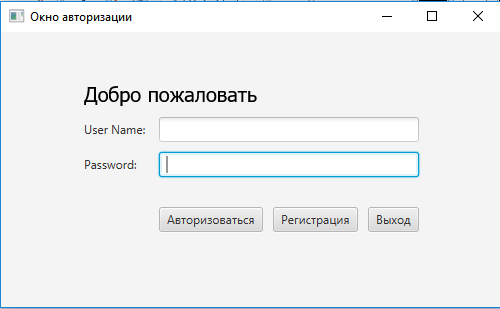
\includegraphics[scale=0.5]{img/login_form.png}
   		\caption{Окно авторизации}
   		\label{fig:login_form}
    \end{figure}
\end{center}
\begin{center}
	\begin{figure}[h!]
		\centering
   		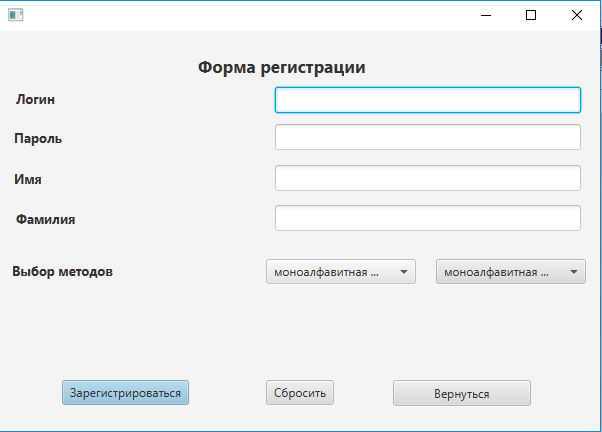
\includegraphics[scale=0.5]{img/registry_form.png}
   		\caption{Окно регистрации}
   		\label{fig:registry_form}
    \end{figure}
\end{center}
\par После прохождения авторизации пользователю открывается главное окно приложения, в котором ему, из списка методов шифрования, будут доступны лишь те методы, которые были выбраны им на этапе регистрации (рис. \ref{fig:main_form}).
\begin{center}
	\begin{figure}[h!]
		\centering
   		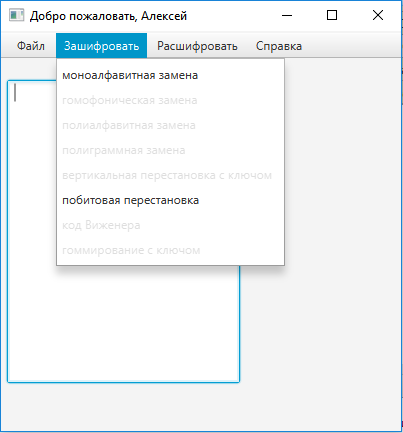
\includegraphics[scale=0.5]{img/main_form.png}
   		\caption{Главное окно программы}
   		\label{fig:main_form}
    \end{figure}
\end{center}

\begin{center}
	\begin{figure}[h!]
		\centering
   		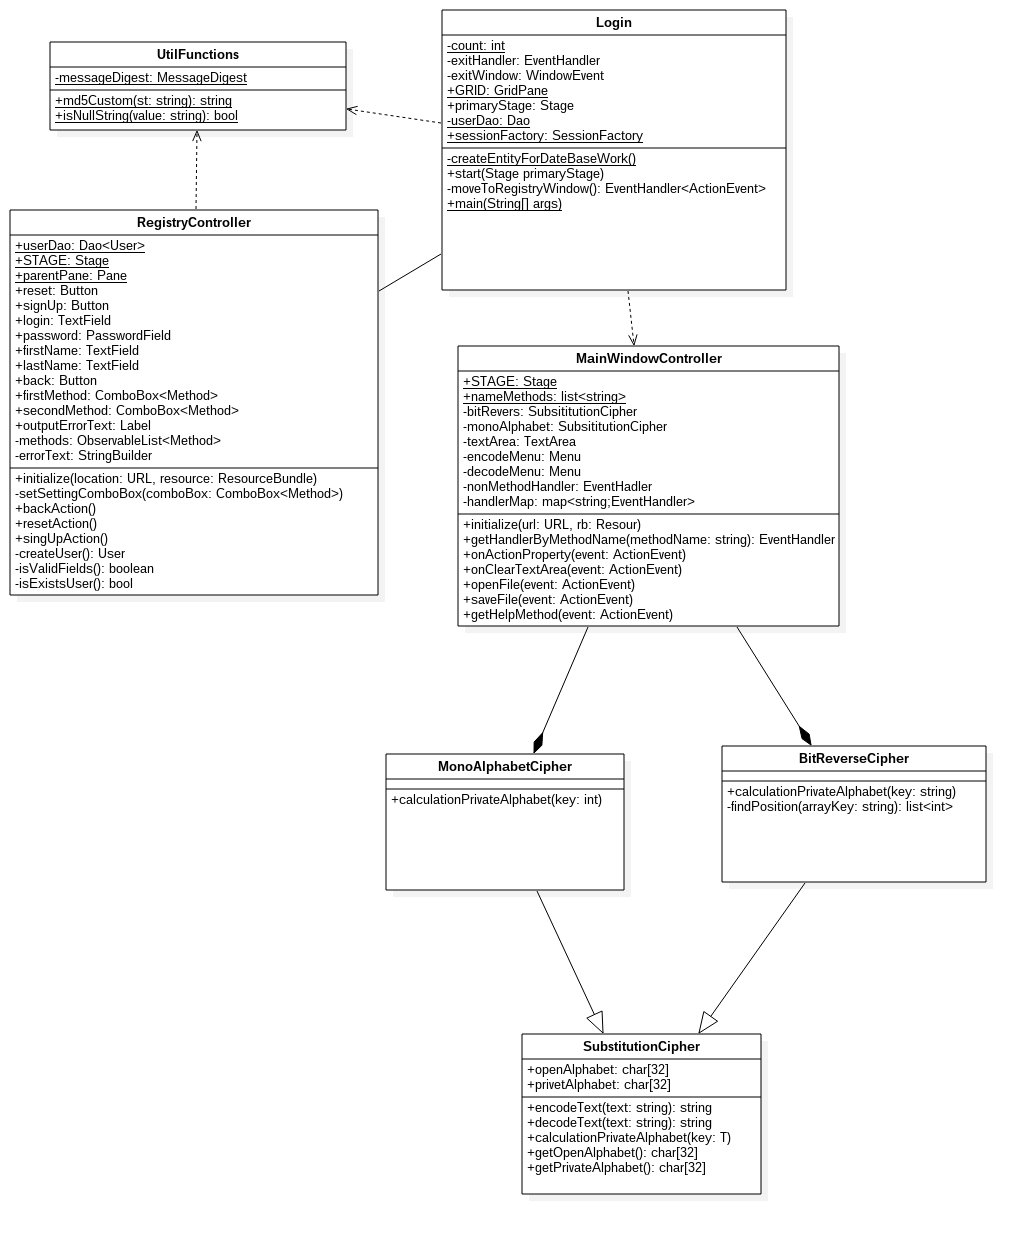
\includegraphics[scale=0.5]{img/class_diagram.png}
   		\caption{Диаграмма классов проекта}
   		\label{fig:class_diagram}
    \end{figure}
\end{center}

\subsection{Ограничения для шифруемого/расшифруемого текста}
Текст принимаемый методами шифрования состоит из строчных букв русского алфавита, из которого изключены буквы 'ё' и 'й', а так же пробел. Оставшиеся символы не входят в состав открытого алфавита, поэтому при их использовании в тексте пользователь увидит следующее сообщение: "Недопустимый символ. Расшифровка/Шифрование не возможно" (Последнее предложение зависит от выбранного пользователем метода. Пример на рис. \ref{fig:wrong_char_and_response}.
\begin{center}
	\begin{figure}[h!]
		\centering
		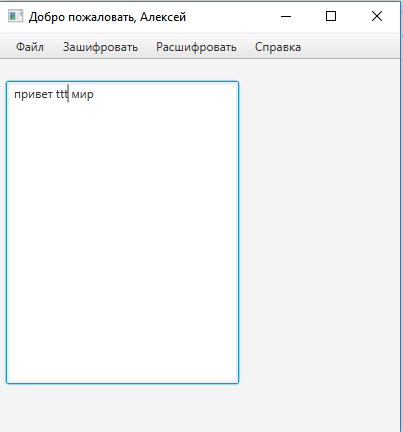
\includegraphics[scale=0.7]{img/wrong_char.png}
		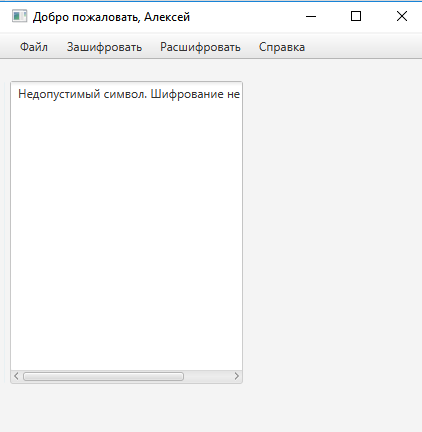
\includegraphics[scale=0.7]{img/wrong_char_response.png}
		\caption{Не верный символ в тексте}
		\label{fig:wrong_char_and_response}
	\end{figure}
\end{center}

\newpage\section{Общее описание тестирования}
В ходе данного тестирования проверяется работа пользовательского GUI как автоматизирванно (с помощью TestFx) так и в ручную. Проверяется работа приложения с базой данных, а также сохранение/загрузка текста в файл.

\par Для проведения тестирования использована библиотека JUnit, а также TestFX, которая нужна для моделирования взаимодействия пользователя с интерфейсом. Для проверки содержимого БД использовался просмотрщик БД ИСР IntellijIdea.

\newpage \section{Модульное тестирование}
\subsection{Общее описание}
Целью модульного тестирования является проверка корректности работы отдельных функций классов программы.
Для его проведения использована библиотека jUnit, а также TestFX для моделирования работы полльзователя с интерфейсом программы (GUI). Для проведения интеграционного были использованы эти же библиотеки, только там уже проверялось взаимодействие классов программы. Поэтому для проведения этих этапов тестирования был разработан общий набор классов для тестирования GUI, который представлен на рисунке \ref{fig:class_diagram_tests_gui}. На диаграмме упущены атрибуты и методы. классов.

\begin{center}
	\begin{figure}[h!]
		\centering
		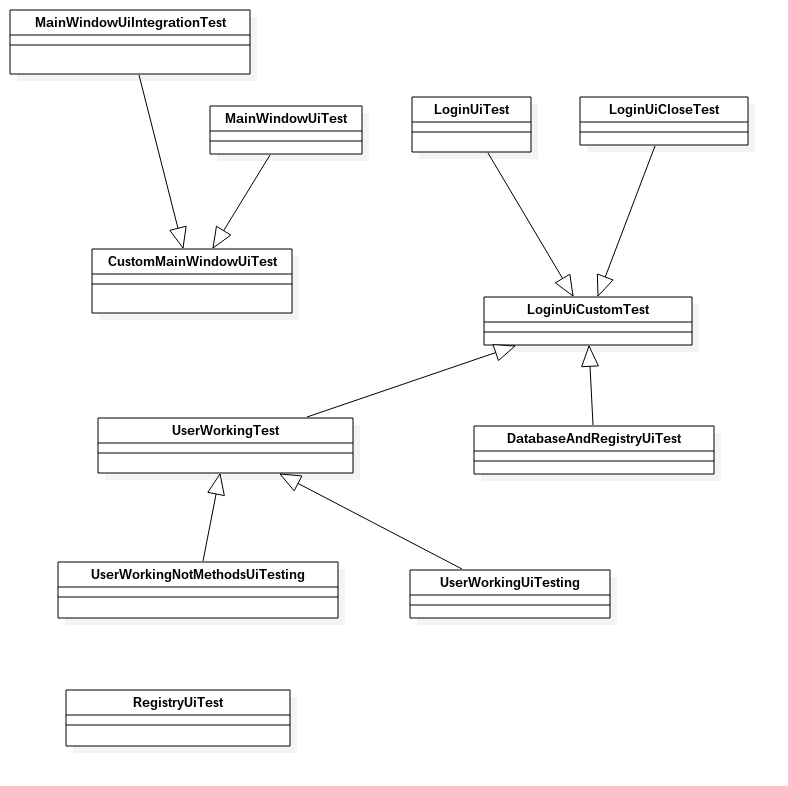
\includegraphics[scale=0.6]{img/class_diagram_ui_tests.png}
		\caption{Диаграмма классов для тестирования GUI}
		\label{fig:class_diagram_tests_gui}
	\end{figure}
\end{center}

Также дополнитеьно для модульного тестирования классов шифрования и регистрации разработаны классы BitReversCipherTest, MonoAlphabetCipherTest и UtilFunctionsTest.

\newpage\subsection{Описание методов и тестов класса MonoAlphabetCipher}
\subsubsection{Метод createOpenAlphabet}
Метод инициализирует массив допустимых символов. Сначала должен быть пробел, потом символы 'a' - 'я' заисключением символов 'ё' и 'й'. Исходный код представлен в листинге \ref{listing:createOpenAlphabet}. Метод унаследован их базового класса.
\begin{lstlisting}[language=java, caption=метод createOpenAlphabet, label = listing:createOpenAlphabet]
	private void createOpenAlphabet() {
        openAlphabet[0] = '\u0020';
        for (int i = 0; i < 9; i++) {
            openAlphabet[i + 1] = (char) ('а' + i);
        }
        for (int i = 10; i < 32; ++i) {
            openAlphabet[i] = (char) ('а' + i);
        }
    }
\end{lstlisting}
Необходимо проверить привильность инициализации, это сделано в листинге \ref{listing:testCalculationPrivateAlphabet}
\subsection{Метод calculationPrivateAlphabet}
Вычисляет закрытый алфавит на основании ключа шифрования (целое число, не превышающее мо модулю $10^9$) (листинг \ref{listing:calculationPrivateAlphabet}). Затем при шифровании символ, имеющий позицию i в OpenAlphabet заменяется символом с этим же номером из массива PrivetAlphabet.
\begin{lstlisting}[language=java, caption=метод calculationPrivateAlphabet, label = listing:calculationPrivateAlphabet]
	@Override
    public void calculationPrivateAlphabet(Integer key) {
        for (int i = 0; i < 32; i++) {
            privateAlphabet[i] = openAlphabet[Math.floorMod(i + key, 32)];
        }
    }
    
\end{lstlisting}
Необходимо проверитть правильность генерации закрытого и открытого алфавита. это делает следующий метод (листинг \ref{listing:testCalculationPrivateAlphabet}). Закрый алфавит созданый по ключу 0 должен совпадать с открытым ключом.
\begin{lstlisting}[language=java, caption=метод теста testCalculationPrivateAlphabet, label = listing:testCalculationPrivateAlphabet]
@Test
    public void testCalculationPrivateAlphabet() {
        char[] actuals = {' ', 'а', 'б', 'в', 'г', 'д', 'е', 'ж', 'з', 'и', 'к', 'л', 'м', 'н', 'о', 'п', 'р', 'с', 'т', 'у', 'ф', 'х', 'ц', 'ч', 'ш', 'щ', 'ъ', 'ы', 'ь', 'э', 'ю', 'я'};
        monoAlphabetCipher.calculationPrivateAlphabet(0);
        assertArrayEquals(monoAlphabetCipher.getPrivateAlphabet(), actuals);
        assertArrayEquals(monoAlphabetCipher.getOpenAlphabet(), actuals);
        assertArrayEquals(monoAlphabetCipher.getOpenAlphabet(), monoAlphabetCipher.getOpenAlphabet());
    }
\end{lstlisting}
Далее проверка генерации закрытого алфавита при ненулевом ключе (листинг \ref{listing:testCalculationPrivateAlphabetCaesarCipher}).
\begin{lstlisting}[language=java, caption=метод теста testCalculationPrivateAlphabet, label = listing:testCalculationPrivateAlphabetCaesarCipher]
	@Test
    public void testCalculationPrivateAlphabetCaesarCipher() {
        char[] actuals = {'в', 'г', 'д', 'е', 'ж', 'з', 'и', 'к', 'л', 'м', 'н', 'о', 'п', 'р', 'с', 'т', 'у', 'ф', 'х', 'ц', 'ч', 'ш', 'щ', 'ъ', 'ы', 'ь', 'э', 'ю', 'я', ' ', 'а', 'б'};
        monoAlphabetCipher.calculationPrivateAlphabet(3);
        assertArrayEquals(monoAlphabetCipher.getPrivateAlphabet(), actuals);
\end{lstlisting}
Тестируем возвращает ли метод исключение при некорректном значении ключа (листинг \ref{listing1:testExceptions}).
\begin{lstlisting}[language=java, caption=методы проверки исключений, label = listing1:testExceptions]
	@Test(expected = NullPointerException.class)
    public void testNullCalculationPrivateAlphabet() {
        monoAlphabetCipher.calculationPrivateAlphabet(null);
    }

    @Test(expected = ClassCastException.class)
    public void testWrongArgumentCalculationPrivateAlphabet() {
        monoAlphabetCipher.calculationPrivateAlphabet("test");
    }
\end{lstlisting}
\subsubsection{Метод encodeText и decodeText}
Выполняют шифрование и дешифрование текста. Эти методы унаследованы из базового класса (листинг \ref{listing1:encodeAndDecode}). Если переданная строка содержит символы, недопустимые в данном алфавите, то метод должен вернуть строку "Недопустимый символ. Шифрование/Дешифрование не возможно".
\begin{lstlisting}[language=java, caption=методы encode и decode, label = listing1:encodeAndDecode]
     /**
     * Закодировать текст
     *
     * @param originalText текст
     * @return закодированный текст
     */
    public String encodeText(String originalText) {
        originalText = originalText.replaceAll("\n", " ").toLowerCase();
        char[] text = originalText.toCharArray();
        char[] result = new char[text.length];
        int index;
        for (int i = 0; i < text.length; i++) {
            index = contains(openAlphabet, text[i]);
            if (index < 0) return "Недопустимый символ. Шифрование не возможно";
            result[i] = privateAlphabet[index];
        }
        return String.valueOf(result);
    }

    /**
     * Раскодировать текст
     *
     * @param originalText текст
     * @return раскодированный текст
     */
    public String decodeText(String originalText) {
        char[] text = originalText.toCharArray();
        char[] result = new char[text.length];
        int index;
        for (int i = 0; i < text.length; i++) {
            index = contains(privateAlphabet, text[i]);
            if (index < 0) return "Недопустимый символ. Расшифровка не возможно";
            result[i] = openAlphabet[index];
        }
        return String.valueOf(result);
    }

    private int contains(char[] chars, char symbol) {
        for (int i = 0; i < chars.length; i++) {
            if (chars[i] == symbol) {
                return i;
            }
        }
        return -1;
    }
\end{lstlisting}
Необходимо проверить корректность шифрования. Это делают следующие методы (листинг \ref{listing1:testEncocodeAndDecode}).
\begin{lstlisting}[language=java, caption=методы проверки корректности шифрования/дешифрования, label = listing1:testEncocodeAndDecode]
    @Test
    public void testEncodeText() {
        monoAlphabetCipher.calculationPrivateAlphabet(3);
        assertEquals(monoAlphabetCipher.encodeText("тест"), "хифх");
    }

    @Test
    public void testEncodeAndDecode() {
        monoAlphabetCipher.calculationPrivateAlphabet(30);
        String encode = monoAlphabetCipher.encodeText("тест");
        assertEquals("тест", monoAlphabetCipher.decodeText(encode));
    }

\end{lstlisting}
А также корректность певедения метода при недопустимой строке (листинг \ref{listing1:testWrongCharInEncodeAndDecodeText}).
\begin{lstlisting}[language=java, caption=методы проверки корректности шифрования/дешифрования, label = listing1:testWrongCharInEncodeAndDecodeText]
    @Test
    public void testWrongCharInEncodeAndDecodeText() {
        monoAlphabetCipher.calculationPrivateAlphabet(1);
        Assert.assertEquals(monoAlphabetCipher.encodeText("tttt"), "Недопустимый символ. Шифрование не возможно");
        Assert.assertEquals(monoAlphabetCipher.encodeText("й"), "Недопустимый символ. Шифрование не возможно");
        Assert.assertEquals(monoAlphabetCipher.encodeText("ё"), "Недопустимый символ. Шифрование не возможно");
        Assert.assertEquals(monoAlphabetCipher.encodeText("-"), "Недопустимый символ. Шифрование не возможно");
        Assert.assertEquals(monoAlphabetCipher.encodeText("+"), "Недопустимый символ. Шифрование не возможно");
        Assert.assertEquals(monoAlphabetCipher.decodeText("tttt"), "Недопустимый символ. Расшифровка не возможно");
        Assert.assertEquals(monoAlphabetCipher.decodeText("й"), "Недопустимый символ. Расшифровка не возможно");
        Assert.assertEquals(monoAlphabetCipher.decodeText("ё"), "Недопустимый символ. Расшифровка не возможно");
        Assert.assertEquals(monoAlphabetCipher.decodeText("-"), "Недопустимый символ. Расшифровка не возможно");
        Assert.assertEquals(monoAlphabetCipher.decodeText("+"), "Недопустимый символ. Расшифровка не возможно");
    }
\end{lstlisting}
\newpage\subsection{Описание методов и тестов класса BitReverseCipher}
Данный класс выполняет шифрование/дешифрование методом побитовой перестановки. Ключём шифрования является строка являющаяся перестановкий "12345", которая задаёт правило перестановки битов для каждого символа. Напимер строка "54312" означает, что 5-й бит будет переставлен на 1 место (нумерация от 1 до 5), 4-й бит на 2-e место, 3-й бит остаётся на месте, 1-й бит идёт на 4 место, 2-й бит на 5-е.
\par Далее описаны методы, которые переопределены у базового класса.
\subsubsection{Метод findPosition}
Метод на основе ключа генерирует массив, с правилами переставки битов в исходных символов (листинг \ref{listing2:findPosition}).
\begin{lstlisting}[language=java, caption=метод findPosition, label=listing2:findPosition]
    private int[] findPosition(String arrayKey) {
        int[] result = new int[arrayKey.length()];
        result[0] = arrayKey.indexOf("1");
        result[1] = arrayKey.indexOf("2");
        result[2] = arrayKey.indexOf("3");
        result[3] = arrayKey.indexOf("4");
        result[4] = arrayKey.indexOf("5");
        return result;
    }
\end{lstlisting}
Корректнгость данного метода проверяется при описанного дальше метода.
\subsubsection{Метод calculationPrivateAlphabet}
Метод генерирует закрытый алфавит. На вход подаётся строка с ключём (листинг \ref{listing2:calculationPrivateAlphabet}).
\begin{lstlisting}[language=java, caption=метод calculationPrivateAlphabet, label=listing2:calculationPrivateAlphabet]
    public void calculationPrivateAlphabet (String key) {
        int[] arrayKey = findPosition(key);
        for (int i = 0; i < 32; i++) {
            StringBuilder stI = new StringBuilder(Integer.toBinaryString(i));
            for (int j = stI.length(); j < 5; j++) {
                stI.insert(0, "0");
            }
            StringBuilder charAlph = new StringBuilder();
            char[] mass = stI.toString().toCharArray();
            for (int anArrayKey : arrayKey) {
                charAlph.append(mass[anArrayKey]);
            }
            int exitI = Integer.parseInt(charAlph.toString(), 2);
            privateAlphabet[i] = openAlphabet[exitI];
        }
    }
\end{lstlisting}

Можно заметить, что шифрование пробела всегда приведёт к пробельному символу(код 0). Для проверки этого разработаен следующий метод (листинг \ref{listing2:testFirstElementPrivateAlphabetAtAnyKey}).
\begin{lstlisting}[language=java, caption=метод calculationPrivateAlphabet, label=listing2:testFirstElementPrivateAlphabetAtAnyKey]
    @Test
    public void testFirstElementPrivateAlphabetAtAnyKey() {
        bitReversCipher.calculationPrivateAlphabet("54321");
        assertEquals(bitReversCipher.getPrivateAlphabet()[0], ' ');
        bitReversCipher.calculationPrivateAlphabet("53241");
        assertEquals(bitReversCipher.getPrivateAlphabet()[0], ' ');
        bitReversCipher.calculationPrivateAlphabet("13425");
        assertEquals(bitReversCipher.getPrivateAlphabet()[0], ' ');
        bitReversCipher.calculationPrivateAlphabet("31245");
        assertEquals(bitReversCipher.getPrivateAlphabet()[0], ' ');
    }
\end{lstlisting}

Далее проверить в целом построение закрытого и открытого алфавита (листинг \ref{listing2:testCalculationPrivateAlphabet}).
\begin{lstlisting}[language=java, caption=метод calculationPrivateAlphabet, label=listing2:testCalculationPrivateAlphabet]
    @Test
    public void testCalculationPrivateAlphabetEqualsOpenAlphabet() {
        char[] actuals = {' ', 'а', 'б', 'в', 'г', 'д', 'е', 'ж', 'з', 'и', 'к', 'л', 'м', 'н', 'о', 'п', 'р', 'с', 'т', 'у', 'ф', 'х', 'ц', 'ч', 'ш', 'щ', 'ъ', 'ы', 'ь', 'э', 'ю', 'я'};
        bitReversCipher.calculationPrivateAlphabet("12345");
        assertArrayEquals(bitReversCipher.getPrivateAlphabet(), actuals);
        assertArrayEquals(bitReversCipher.getOpenAlphabet(), actuals);
        assertArrayEquals(bitReversCipher.getOpenAlphabet(), bitReversCipher.getOpenAlphabet());
    }

    @Test
    public void testCalculationPrivateAlphabet() {
        char[] actuals = {' ', 'р', 'з', 'ш', 'г', 'ф', 'м', 'ь', 'б', 'т', 'к', 'ъ', 'е', 'ц', 'о', 'ю', 'а', 'с', 'и', 'щ', 'д', 'х', 'н', 'э', 'в', 'у', 'л', 'ы', 'ж', 'ч', 'п', 'я'};
        bitReversCipher.calculationPrivateAlphabet("54321");
        assertArrayEquals(bitReversCipher.getPrivateAlphabet(), actuals);
    }
\end{lstlisting}
Затем можно проверить, что при некорректном значии ключа происходят исключения (листинг \ref{listing2:testWrongValueForCalculationPrivateAlphabet}).
\begin{lstlisting}[language=java, caption=метод calculationPrivateAlphabet, label=listing2:testWrongValueForCalculationPrivateAlphabet]
    @Test(expected = IndexOutOfBoundsException.class)
    public void testWrongValueForCalculationPrivateAlphabet() {
        bitReversCipher.calculationPrivateAlphabet("00000");
    }

    @Test(expected = ClassCastException.class)
    public void testWrongArgumentForCalculationPrivateAlphabet() {
        bitReversCipher.calculationPrivateAlphabet(1213234);
    }
\end{lstlisting}

\subsubsection{Тестирование остальных методов}

Далее необходимо проверить правальность шифрования и расшифрования строки (листинг \ref{listing2:testEncodeDecode}).
\begin{lstlisting}[language=java, caption=метод calculationPrivateAlphabet, label=listing2:testEncodeDecode]
	@Test
    public void testEncode() {
        bitReversCipher.calculationPrivateAlphabet("54321");
        assertEquals(bitReversCipher.encodeText("тест"), "имси");
    }

    @Test
    public void testEncodeDecode() {
        bitReversCipher.calculationPrivateAlphabet("54321");
        String encode = bitReversCipher.encodeText("тест");
        assertEquals(bitReversCipher.decodeText(encode), "тест");
    }
\end{lstlisting}
Проверка поведения при некоректном шифруемом/дешифруемом тексте (листинг \ref{listing2:testWrongCharInEncodeAndDecodeText}).
\begin{lstlisting}[language=java, caption=метод calculationPrivateAlphabet, label=listing2:testWrongCharInEncodeAndDecodeText]
    @Test
    public void testWrongCharInEncodeAndDecodeText() {
        bitReversCipher.calculationPrivateAlphabet("54321");
        Assert.assertEquals(bitReversCipher.encodeText("tttt"), "Недопустимый символ. Шифрование не возможно");
        Assert.assertEquals(bitReversCipher.encodeText("й"), "Недопустимый символ. Шифрование не возможно");
        Assert.assertEquals(bitReversCipher.encodeText("ё"), "Недопустимый символ. Шифрование не возможно");
        Assert.assertEquals(bitReversCipher.encodeText("-"), "Недопустимый символ. Шифрование не возможно");
        Assert.assertEquals(bitReversCipher.encodeText("+"), "Недопустимый символ. Шифрование не возможно");
        Assert.assertEquals(bitReversCipher.decodeText("tttt"), "Недопустимый символ. Расшифровка не возможно");
        Assert.assertEquals(bitReversCipher.decodeText("й"), "Недопустимый символ. Расшифровка не возможно");
        Assert.assertEquals(bitReversCipher.decodeText("ё"), "Недопустимый символ. Расшифровка не возможно");
        Assert.assertEquals(bitReversCipher.decodeText("-"), "Недопустимый символ. Расшифровка не возможно");
        Assert.assertEquals(bitReversCipher.decodeText("+"), "Недопустимый символ. Расшифровка не возможно");
    }
\end{lstlisting}


\newpage \section{Интеграционное тестирование}
\subsection{Общее описание}
Целью интеграционного тестирования является проверка всех возможных непосредвенных взаимодействий классов программы

\newpage \section{Системное тестирование}
\subsection{Общее описание}
Целью является тестирование всей системы в целом на реальной БД.

\newpage\section*{Выводы}
\addcontentsline{toc}{section}{Выводы}
В ходе выполнения лабораторной работы было разработано и проведено системное тестирвание пректа. Для написания тестов была использована библиотека JUnit, а действия пользователя моделировались с помошью библиотеки TestFX. Ручные тесты составлялись из рассчёта на то, чтобы смоделировать типовые действие пользователя, которые не были протестированы на предыдущем этапе. В ходе тестирования ошибок не обнаружено.

\newpage\section*{Приложения}
\addcontentsline{toc}{section}{Приложения}


\end{document}